% Developing a digital synthesizer in C++

\documentclass[12pt,twoside]{report}

\usepackage{listings}

\usepackage{color}

\usepackage{url}

\usepackage{graphicx}

\usepackage{newtxtext}

\usepackage[labelfont=bf]{caption}

\usepackage[a4paper,margin=1in]{geometry}

\usepackage{fancyhdr}

\usepackage{mathtools}

\usepackage{gensymb}

\usepackage{multicol}

\usepackage{floatrow}

\begin{document}

\everymath{\displaystyle}

\fancyhf{}
%\renewcommand{\headrulewidth}{0pt}
\fancyhead[LO]{\leftmark}
\fancyhead[RE]{SECTION \rightmark}
\fancyhead[RO,LE]{\thepage}

\pagestyle{fancy}

\definecolor{custommagenta}{RGB}{230,70,165}
\definecolor{customgreen}{RGB}{30,210,100}
\definecolor{customgray}{gray}{0.5}

\lstset{
% Format settings
language=C++,
tabsize=4,
breakatwhitespace=true,
breaklines=true,
frame=leftline,
captionpos=b,
keepspaces=true,
showstringspaces=false,
numbers=left,
numberstyle=\scriptsize,
% Style settings
basicstyle=\ttfamily\scriptsize,
keywordstyle=\color{custommagenta}\ttfamily,
stringstyle=\color{customgreen}\ttfamily,
commentstyle=\color{customgray}\ttfamily,
morecomment=[l][\color{red}]{\#}
}

% Macro for source code inclusion. Moves to main
% directory then takes the further path as argument
\newcommand{\code}[2][1]{\lstinputlisting[firstnumber=#1]{#2}}

\newcommand{\citebs}[1]{(Mitchell, 2008, p. #1)}

\newcommand{\citedsp}[1]{(Smith, 1999, p. #1)}

\newcommand{\sidecap}[3]{\floatbox[{\capbeside\thisfloatsetup{capbesideposition={right,center}}}]{table}[\FBwidth]{\caption{#1} \label{#2}}{#3}}

\title{Developing a Digital Synthesizer in C++}

\author{
Peter Goldsborough\\
\texttt{petergoldsborough@hotmail.com}
}

\date{\today}

\maketitle

\tableofcontents

\chapter{Sound in the Digital Realm}

\section{What is a Music Synthesizer?}



\section{From Analog to Digital}

Our everyday experience of sound is an entirely analog one. When a physical     object emits or reflects a sound wave into space and towards our ears, the signal produced consists of an infinite set of values, spaced apart in infinitesimal intervals. Due to the fact that such a signal has an amplitude value at every single point in time, it is called a continuous signal. \citedsp{11} Figure \ref{fig:cont} displays the continuous representation of a sine wave.

\begin{figure}[h!]

  \centering

  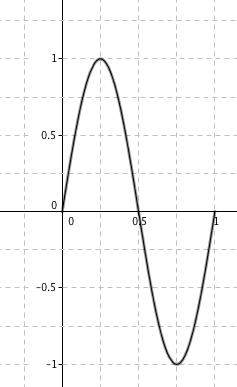
\includegraphics[scale=0.5]{img/cont}

  \caption{The continuous representation of a typical sine wave. In this case, both the signal's frequency $f$ as well as the maximum elongation from the equilibrium $a$ are equal to $1$. }

  \label{fig:cont}

\end{figure}

\pagebreak

While continuous signals and the idea of an infinite, uncountable set of values are easy to model in mathematics and physics --- the analog world, computers --- in the digital world --- effectively have no means by which to represent something that is infinite, since computer memory is a finite resource. Therefore, signals in the digital domain are discrete, meaning they are composed of periodic \emph{samples}. A sample is a discrete recording of a continuous signal's amplitude, taken in a constant time interval \citebs{16}. The process by which a continuous signal is converted to a discrete signal is called \emph{quantization}, \emph{digitization} or simply \emph{analog-to-digital-conversion} \citedsp{35-36} \citebs{16}. The reverse process of converting discrete samples to a continuous signal is called \emph{digital-to-analog-conversion} \citebs{17}. Figure \ref{fig:disc} shows the discrete representation of a sine wave, the same signal that was previously shown as a continuous signal in Figure \ref{fig:cont}.

\begin{figure}[h!]

  \centering

  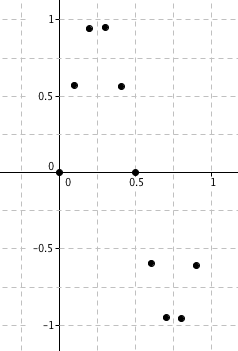
\includegraphics[scale=0.5]{img/disc}

  \caption{The discrete representation of a typical sine wave.}

  \label{fig:disc}

\end{figure}

\section{Sample Rate}

The sample rate (often referred to as sampling rate or sampling frequency), commonly denoted by $f_{s}$, is the rate at which samples of a continuous signal are taken. The value of the sample rate is given in Hertz (Hz) or samples-per-second. Common values for audio sampling rates are 44.1 kHz, a frequency originally chosen by Sony in 1979 that is still used for Compact Discs, and 48 kHz, the standard audio sampling rate used today \citebs{18} (Colletti, 2013). The reciprocal of the sample rate yields the sampling interval, denoted by $T_{s}$ and measured in seconds, which is the time period after which a single sample is taken from a continuous signal:\begin{center} $T_{s} = \frac{1}{f_{s}}$ \end{center} The reciprocal of the sample interval again yields the sampling rate: \begin{center} $f_{s} = \frac{1}{T_{s}}$ \end{center}

\section{Nyquist limit}

The sample rate determines the range of frequencies that can be represented by a digital sound system, as only frequencies that are less than or equal to one half of the sampling rate, where it is possible to take at least one sample above the equilibrium and at least one sample below the equilibrium for every cycle \citebs{18}, can be "properly sampled". To sample a signal "properly" means to be able to "reconstruct" a continuous signal, given a set of discrete samples, "exactly", i.e. without any \emph{quantization errors}. The value of one half of the sample rate is called the \emph{Nyquist frequency} or \emph{Nyquist limit}, named after Harry Nyquist, who first described the Nyquist limit and associated phenomena together with Claude Shannon in the 1940s, stating that "a continuous signal can be properly sampled, only if it does not contain frequency components above one half the sampling rate" \citedsp{40}. Any frequencies above the Nyquist limit lead to \emph{aliasing}, which is discussed in the next section.\\

Given the definition of the Nyquist limit and considering the fact that the limit of human hearing is approximately 20 kHz (Cutnell \& Johnson, 1998, p. 466), the reason for which the two most common audio sample rates are 40 kHz and above is clear: they were chosen to allow the "proper" representation of the entire audio frequency range, since a sample rate of 40 kHz meets the Nyquist requirement of a sample rate at least twice the maximum frequency component of the signal to be sampled (the Nyquist limit), in this case ca. 20 Khz.

\section{Aliasing}

When a signal's frequency exceeds the Nyquist limit, it is said to produce an \emph{alias}, a new signal with a different frequency that is indistinguishable from the original signal when sampled. This is due to the fact that a signal with a frequency component above the Nyquist limit no longer has one sample taken above and one below the zero level for each cycle, but at arbitrary points of the original signal, which, when reconstructed, yield an entirely different signal. For example, if the sinusoid depicted in Figure \ref{fig:orig}, with a frequency of 4 Hz, is sampled at a sample rate of 5 samples per second, shown in Figure \ref{fig:sampled} meaning the frequency of the continuous signal is higher than the Nyquist limit (here 2.5 Hz), the reconstructed signal, approximated in Figure \ref{fig:approx}, will look completely different from the original sinusoid. "This phenomenon of [signals] changing frequency during sampling is called aliasing, [...] an example of improper sampling" \citedsp{40}.

\begin{figure}[b!]

  \centering

  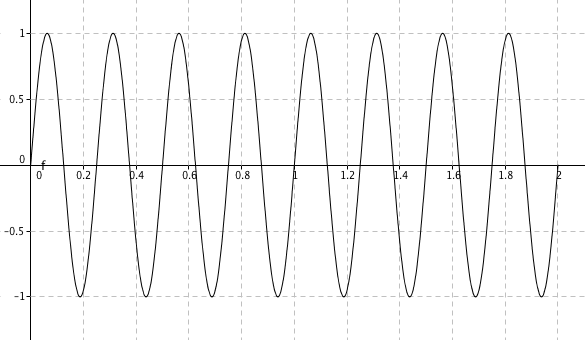
\includegraphics[scale=0.5]{img/orig}

  \caption{A sinusoid with a frequency of 4 Hz.}

  \label{fig:orig}

\end{figure}

\begin{figure}

  \centering

  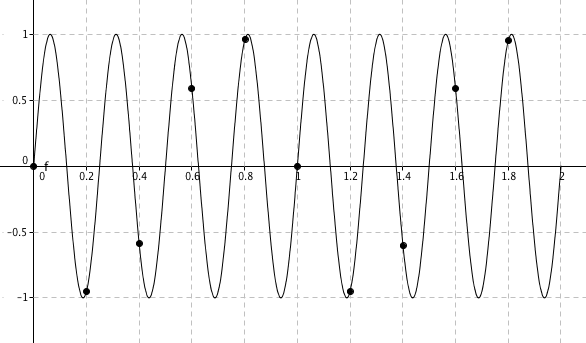
\includegraphics[scale=0.5]{img/sampled}

  \caption{A sinusoid with a frequency of 4 Hz, sampled at a sample rate of 5 Hz. According to the Nyquist Theorem, this signal is sampled improperly, as the frequency of the continuous signal is not less than or equal to one half of the sample rate, in this case 2.5 Hz. }

  \label{fig:sampled}

\end{figure}

\begin{figure}

  \centering

  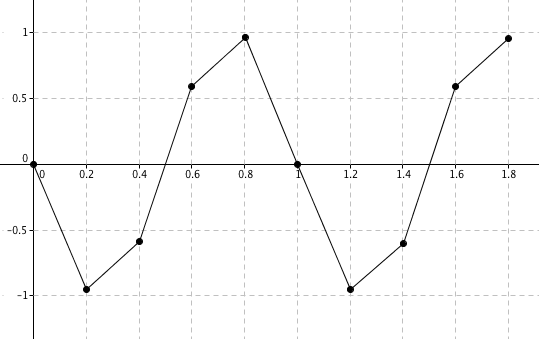
\includegraphics[scale=0.5]{img/approx}

  \caption{An approximated representation of the signal created from the sampling process shown in Figure \ref{fig:sampled}. Visually as well as acoustically, the new signal is completely different from the original signal. However, in terms of sampling, they are indistinguishable from each other due to improper sampling. These signals are said to be \emph{aliases} of each other.}

  \label{fig:approx}

\end{figure}

\section{Overflow}

Another interesting property of digital sound, which is not encountered in the analog world, is that it can overflow. When we attempt to increase the loudness of something in the analog world, e.g. by hitting a drum more intensely, the expected result is a louder sound. In the digital realm however, it may occur that attempting to increase a signal's amplitude does not result in an increased loudness, but in distortion. The cause of this phenomenon lies in the way digital audio is stored. Since computer memory is a finite resource, each sample has a dedicated portion of computer memory allocated to it. For example, the Waveform Audio File Format (WAVE), a common computer file format for audio data, stores each sample of an audio track as a 16-bit signed integer. A 16-bit signed integer gives a possible range of $-2^{16-1}$ to $2^{16-1}$ ($16-1$ because the most significant bit is used as the sign bit in two's complement representation). This means that a signal with an amplitude of 1 will be stored as 32767, an amplitude of 0.5 as 16384, an amplitude of -1 as -32768 and so on. If one tries to increase the amplitude of a signal whose value has already saturated the available range and space allocated to it, in this case 32767 on the positive end and -32768 on the negative end, the result is that the integer with which the sample is stored \emph{overflows}. Because WAVE files (and many other storage media) store samples as \emph{signed} integers, overflow always results in a change of sign:

$$32767_{10} = 0111111111111111_{2}$$
$$0111111111111111_{2} + 1 = 1000000000000000_{2} = -32768_{10}$$
$$1000000000000000_{2} - 1 = 0111111111111111_{2} = 32767_{10}$$

A visualization of the result of increasing the amplitude of a signal with a saturated value (an amplitude of 1), shown in Figure \ref{fig:no-over}, is given in Figure \ref{fig:over}.

\begin{figure}[h!]
  \centering
  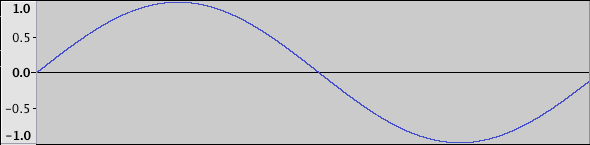
\includegraphics[scale=0.5]{img/no-over}
  \caption{A typical sinusoidal signal with an amplitude of 1. The integer range provided by the allocated memory for the top-most sample is saturated, meaning it is equal to $32767_{10}$ or $0111111111111111_{2}$.}
  \label{fig:no-over}
\end{figure}

\begin{figure}[h!]
  \centering
  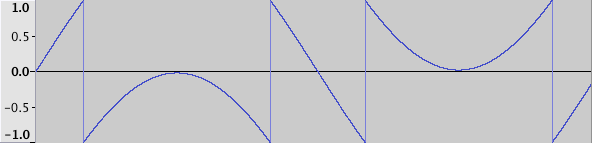
\includegraphics[scale=0.5]{img/over}
  \caption{What happens when the amplitude of the signal from Figure \ref{fig:no-over} is increased by a factor of 2. Multiple samples have overflowed and thus changed their sign. Because of the way two's-complement representation is implemented, the signal continues it's path as if no overflow had ever occurred. The only difference being, of course, that the sign has changed mid-way. }
  \label{fig:over}
\end{figure}

\chapter{Generating Sound}

The following sections will outline how digital sound can be generated in theory and implemented in practice, using the C++ programming language.

\section{Simple Waveforms}

The simplest possible waveform is the sine wave. As a function of time, it can be mathematically represented by Equation \ref{eq:sine}, where $A$ is the maximum amplitude of the signal, $f$ the frequency in Hertz and $\phi$ an initial phase offset in radians:

\begin{equation}
  f_{s}(t) = A \sin(2 \pi  f t + \phi)
  \label{eq:sine}
\end{equation}

A computer program to compute the values of a sine wave with a variable duration, implemented in C++, is shown in Table \ref{code:sine}. Another waveform similar to the sine wave is the cosine wave, which differs only in a phase offset of 90\degree or $\frac{\pi}{2}$ radians:\\
\begin{equation}
  f_{c}(t) = A \cos(2 \pi  f t + \phi) = A \sin(2 \pi f t + \phi + 90)
  \label{eq:cosine}
\end{equation}\\
Therefore, the program from Table \ref{code:sine} could be modified to compute a cosine wave by changing line 22 from:\\

\begin{lstlisting}[firstnumber=22]
  double phase = 0;
\end{lstlisting}
to
\begin{lstlisting}[firstnumber=22]
  double phase = pi/2.0;
\end{lstlisting}

\begin{table}[p!]
  \code{code/sine.cpp}
  \label{code:sine}
  \caption{C++ implementation of a complete sine wave generator.}
\end{table}

\section{Complex Waveforms}

Now that the process of creating simple sine and cosine waves has been discussed, the generation of more complex waveforms can be examined. Generally, there are two methods by which complex waveforms can be created in a digital synthesis system: mathematical calculation or additive synthesis.

\subsection{Mathematical Calculation of Complex Waveforms}

In the first case --- mathematical calculation, waveforms are computed according to certain mathematical formulae and thus yield \emph{perfect} or \emph{exact} waveforms, such as a square wave that is equal to the maximum amplitude exactly one half of a period and equal to the minimum amplitude for the rest of the period. While these waveforms produce a very crisp and clear sound, they are rarely found in nature due to their degree of perfection and are consequently rather undesirable for a music synthesizer. Nevertheless, they are considerably useful for modulating other signals, as tiny acoustical imperfections such as those found in additively synthesized waveforms can result in unwanted distortion which is not encountered when using mathematically calculated waveforms. Therefore, exact waveforms are the best choice for modulation sources such as Low Frequency Oscillators (LFOs), which are discussed in later chapters. \citebs{71}\\\\
The following paragraphs will analyze how four of the most common waveforms found in digital synthesizers, the square, the sawtooth, the ramp and the triangle wave, can be generated via mathematical calculation.\\\\
\emph{Note: There have found to be disparities in literature over which waveform is a sawtooth and which a ramp wave. This thesis will consider a sawtooth wave as descending from maximum to minimum amplitude with time and a ramp wave as ascending from minimum to maximum amplitude with time.}

\subsubsection{Square Waves}

Ideally, a square wave is equal to its maximum amplitude for exactly one half of a period and equal to its minimum amplitude for the other half of the same period. A single period of a square wave can be calculated as shown in Equation \ref{eq:dsquare1}, where the independent variable $t$ as well as the period $T$ can be either in samples or in seconds. A mathematical Equation for a full, periodic square wave function is given by Equation \ref{eq:dsquare2}, where $t$ is time in seconds and the frequency $f$ in Hertz. An equivalent C++ computer program is shown in Table \ref{code:dsquare}.

\begin{multicols}{2}

  \begin{equation}
    f(t) =
    \begin{cases}
      1,& \text{if } 0 \leq t < \frac{T}{2}\\
      -1,& \text{if } \frac{T}{2} \leq t < T
    \end{cases}
    \label{eq:dsquare1}
  \end{equation}

  \begin{equation}
    f(t) =
    \begin{cases}
      1,& \text{if } \sin(2 \pi f t) > 0\\
      -1,& \text{otherwise}
    \end{cases}
    \label{eq:dsquare2}
  \end{equation}

\end{multicols}

\begin{table}
  \sidecap{C++ code to generate and return one period of a square wave, where \texttt{period} is the period duration in samples. Note that this function increments in sample time, measured in seconds, rather than actual samples. This prevents a one-sample quantization error at the mid-point, since time can always be halved whereas a sample is a fixed entity and cannot be broken down any further.}{code:dsquare}{\code{code/dsquare.cpp}}
\end{table}

\subsubsection{Sawtooth Waves}

An ideal sawtooth wave descends from its maximum amplitude to its minimum amplitude linearly before jumping back to the maximum amplitude at the beginning of the next period. A mathematical Equation for a single period of such a sawtooth wave function, calculated directly from the phase, is given by Equation \ref{eq:dsaw1} \citebs{68}. Alternatively, the function can depend on time or on samples, as shown by Equation \ref{eq:dsaw2}, where $T$ is the period. A computer program to compute one period of a sawtooth wave is given in Table \ref{code:dsaw}.

\begin{multicols}{2}

    \begin{equation}
      f(\phi) =
      \begin{cases}
        -\frac{\phi}{\pi} + 1,& \text{if } 0 \leq \phi < 2 \pi
      \end{cases}
      \label{eq:dsaw1}
    \end{equation}

    \begin{equation}
      f(t) =
      \begin{cases}
        -\frac{2t}{T} + 1,& \text{if } 0 \leq t < 1
      \end{cases}
      \label{eq:dsaw2}
    \end{equation}

\end{multicols}

\begin{table}
  \sidecap{C++ code to generate one period of a sawtooth wave function, where \texttt{period} is the period duration in samples.}{code:dsaw}{\code{code/dsaw.cpp}}
\end{table}

\subsubsection{Ramp Waves}

A ramp wave is, quite simply, an inverted sawtooth wave. It ascends from its minimum amplitude to its maximum amplitude linearly, after which it jumps back down to the minimum amplitude. Consequently, Equation  \ref{eq:dramp1} and \ref{eq:dramp2} differ from sawtooth Equation  \ref{eq:dsaw1} and \ref{eq:dsaw2} only in their sign and offset. The equivalent C++ implementation shown in Table \ref{code:dramp} also reflects these differences.

\begin{multicols}{2}

  \begin{equation}
    f(\phi) =
    \begin{cases}
      \frac{\phi}{\pi} - 1,& \text{if } 0 \leq \phi < 2 \pi
    \end{cases}
    \label{eq:dramp1}
  \end{equation}

  \begin{equation}
    f(t) =
    \begin{cases}
      \frac{2t}{T} - 1,& \text{if } 0 \leq t < 1
    \end{cases}
    \label{eq:dramp2}
  \end{equation}

\end{multicols}

\begin{table}
  \sidecap{C++ ramp wave generator. This code differs from the program shown in Table \ref{code:dsaw} solely in the amplitude offset (-1 instead of 1) and the increment, which is now positive. }{code:dramp}{\code{code/dramp.cpp}}
\end{table}

\pagebreak

\subsubsection{Triangle waves}

A triangle wave can be seen as a combination of a ramp wave and a sawtooth wave, or as a linear, "edgy", sine wave. It increments from its minimum amplitude to its maximum amplitude linearly one half of a period and decrements back to the minimum during the other half. Simply put, "[a] triangle wave is a linear increment or decrement that switches direction every $\pi$ radians" \citebs{69}. A mathematical definition for one period of a triangle wave is given by Equation  \ref{eq:dtri1}, where $\phi$ is the phase in radians. If $\phi$ is kept in the range of $[-\pi;\pi]$ rather than the usual range of $[0;2 \pi]$, the subtraction of $\pi$ can be eliminated, yielding Equation  \ref{eq:dtri2}. If the dependent variable is time, in seconds, or samples, Equation  \ref{eq:dtri3} can be used for a range of $[0;T]$, where $T$ is the period, and Equation  \ref{eq:dtri4} for a range of $[-\frac{T}{2};\frac{T}{2}]$. A C++ implementation is shown in Table \ref{code:dtri}.

\begin{multicols}{2}

  \begin{equation}
    f(\phi) =
    \begin{cases}
      1 - \frac{2 |\phi - \pi|}{\pi},& \text{if } 0 \leq \phi < 2 \pi
    \end{cases}
    \label{eq:dtri1}
  \end{equation}

  \begin{equation}
    f(\phi) =
    \begin{cases}
      1 - \frac{2 |\phi|}{\pi},& \text{if } -\pi \leq \phi < \pi
    \end{cases}
    \label{eq:dtri2}
  \end{equation}

\end{multicols}

\begin{multicols}{2}

  \begin{equation}
    f(t) =
    \begin{cases}
      1 - \frac{4 |t - \frac{T}{2}|}{T},& \text{if } 0 \leq t < 1
    \end{cases}
    \label{eq:dtri3}
  \end{equation}

  \begin{equation}
    f(t) =
    \begin{cases}
      1 - \frac{4 |t|}{T},& \text{if } -\frac{T}{2} \leq t < \frac{T}{2}
    \end{cases}
    \label{eq:dtri4}
  \end{equation}

\end{multicols}

\begin{table}
  \sidecap{C++ program to compute one period of a triangle wave.}{code:dtri}{\code{code/dtri.cpp}}
\end{table}

\subsection{Additive Synthesis}

The second method of generating complex waveforms, Additive Synthesis, produces waveforms that, despite not being mathematically perfect, are closer to the waveforms found naturally. This method involves the summation of a theoretically infinite, practically finite set of sine and/or cosine waves with varying parameters and is often called Fourier Synthesis, after the 18th century French scientist, Joseph Fourier, who first described the process and associated phenomena of summing sine and cosine waves to produce complex waveforms. This calculation of a complex, periodic waveform from a sum of sine and cosine functions is also called a Fourier Transform or a Fourier Series, both part of the Fourier Theorem. In a Fourier Series, a single sine/cosine component is either called a harmonic, an overtone or a partial. All three name the same idea of a waveform with a frequency that is an \emph{integer multiple} of some fundamental pitch or frequency. \citebs{64} Throughout this thesis the term \emph{partial} will be preferred. \\\\Equation 2.13 gives the general definition of a discrete Fourier Transform. Equation 2.14 shows a simplified version of Equation 2.13. Table \ref{code:partial} presents a C++ struct to represent a single partial and Tables \ref{code:add1} and \ref{code:add2} a piece of C++ code to compute one period of any Fourier Series.

\begin{figure}[h!]
  $f(t) = \frac{a_{0}}{2} + \sum\limits_{n=1}^\infty (a_{n} \cos(\omega n t) = b_{n} \sin(\omega n t))$
  \caption*{\textbf{Equation 2.13: }Formula to calculate an infinite Fourier series, where $\frac{a_{n}}{2}$ is the center amplitude, $a_{n}$ and $b_{n}$ the partial amplitudes and $\omega$ the angular frequency, which is equal to $2 \pi f$.}
  \label{fig:fourier1}
\end{figure}

\begin{figure}[h!]
  $f(t) = \sum\limits_{n=1}^N a_{n} \sin(\omega n t + \phi_{n})$
  \caption*{\textbf{Equation 2.14:} Simplificiation of Equation 2.13. Note the change from a computationally impossible infinite series to a more practical finite series. Because a cosine wave is a sine wave shifted by 90\degree or $\frac{\pi}{2}$ radians, the $\cos$ function can be eliminated and replaced by an appropiate $\sin$ function with a phase shift $\phi_{n}$.}
  \label{fig:fourier2}
\end{figure}

\begin{table}
  \sidecap{C++ code to represent a single partial in a Fourier Series.}{code:partial} {\code{code/partial.cpp}}
\end{table}

\begin{table}
  \sidecap{}{code:add1}{\code{code/add1.cpp}}
\end{table}

\begin{table}
  \sidecap{\emph{Continuation of Table \ref{code:add1}}. C++ program to produce one period of an additively synthesized complex waveform, given a start and end iterator to a container of partials, a buffer length, a maximum, "master", amplitude, a boolean whether or not to apply sigma approximation and lastly a maximum bit width parameter.}{code:add2}{\code[56]{code/add2.cpp}}
\end{table}

\noindent The following paragraphs will examine how the four waveforms presented in Section 2.2.1, the square, the sawtooth, the ramp and the triangle wave, can be synthesized additively.

\subsubsection{Square Waves}

When speaking of Additive or Fourier Synthesis, a square wave is the result of summing all odd-numbered partials (3rd, 5th, 7th etc.) at a respective amplitude equal to the reciprocal of their partial number ($\frac{1}{3}$, $\frac{1}{5}$, $\frac{1}{7}$ etc.). The amplitude of each partial must decrease with increasing partial numbers to prevent amplitude overflow. A mathematical equation for such a square wave with $N$ partials is given by Equation \ref{eq:asquare}, where $2n - 1$ makes the series use only odd partials. A good maximum number of partials $N$ for near-perfect but still naturally sounding waveforms is 64, a value determined empirically. Higher numbers do not produce significant improvements in sound quality. Table \ref{code:asquare} displays the C++ code needed to produce one period of a square wave in conjuction with the \texttt{additive} function from Tables \ref{code:add1} and \ref{code:add2}. Figure \ref{fig:square} shows the result of summing 2, 4, 8, 16, 32 and finally 64 partials.

\begin{equation}
  f(t) = \sum\limits_{n=1}^N \frac{1}{2n -1} \sin(\omega (2n - 1) t)
  \label{eq:asquare}
\end{equation}

\begin{figure}

  \CenterFloatBoxes

  \begin{floatrow}

    \ffigbox{\caption{} \label{fig:square}}{ 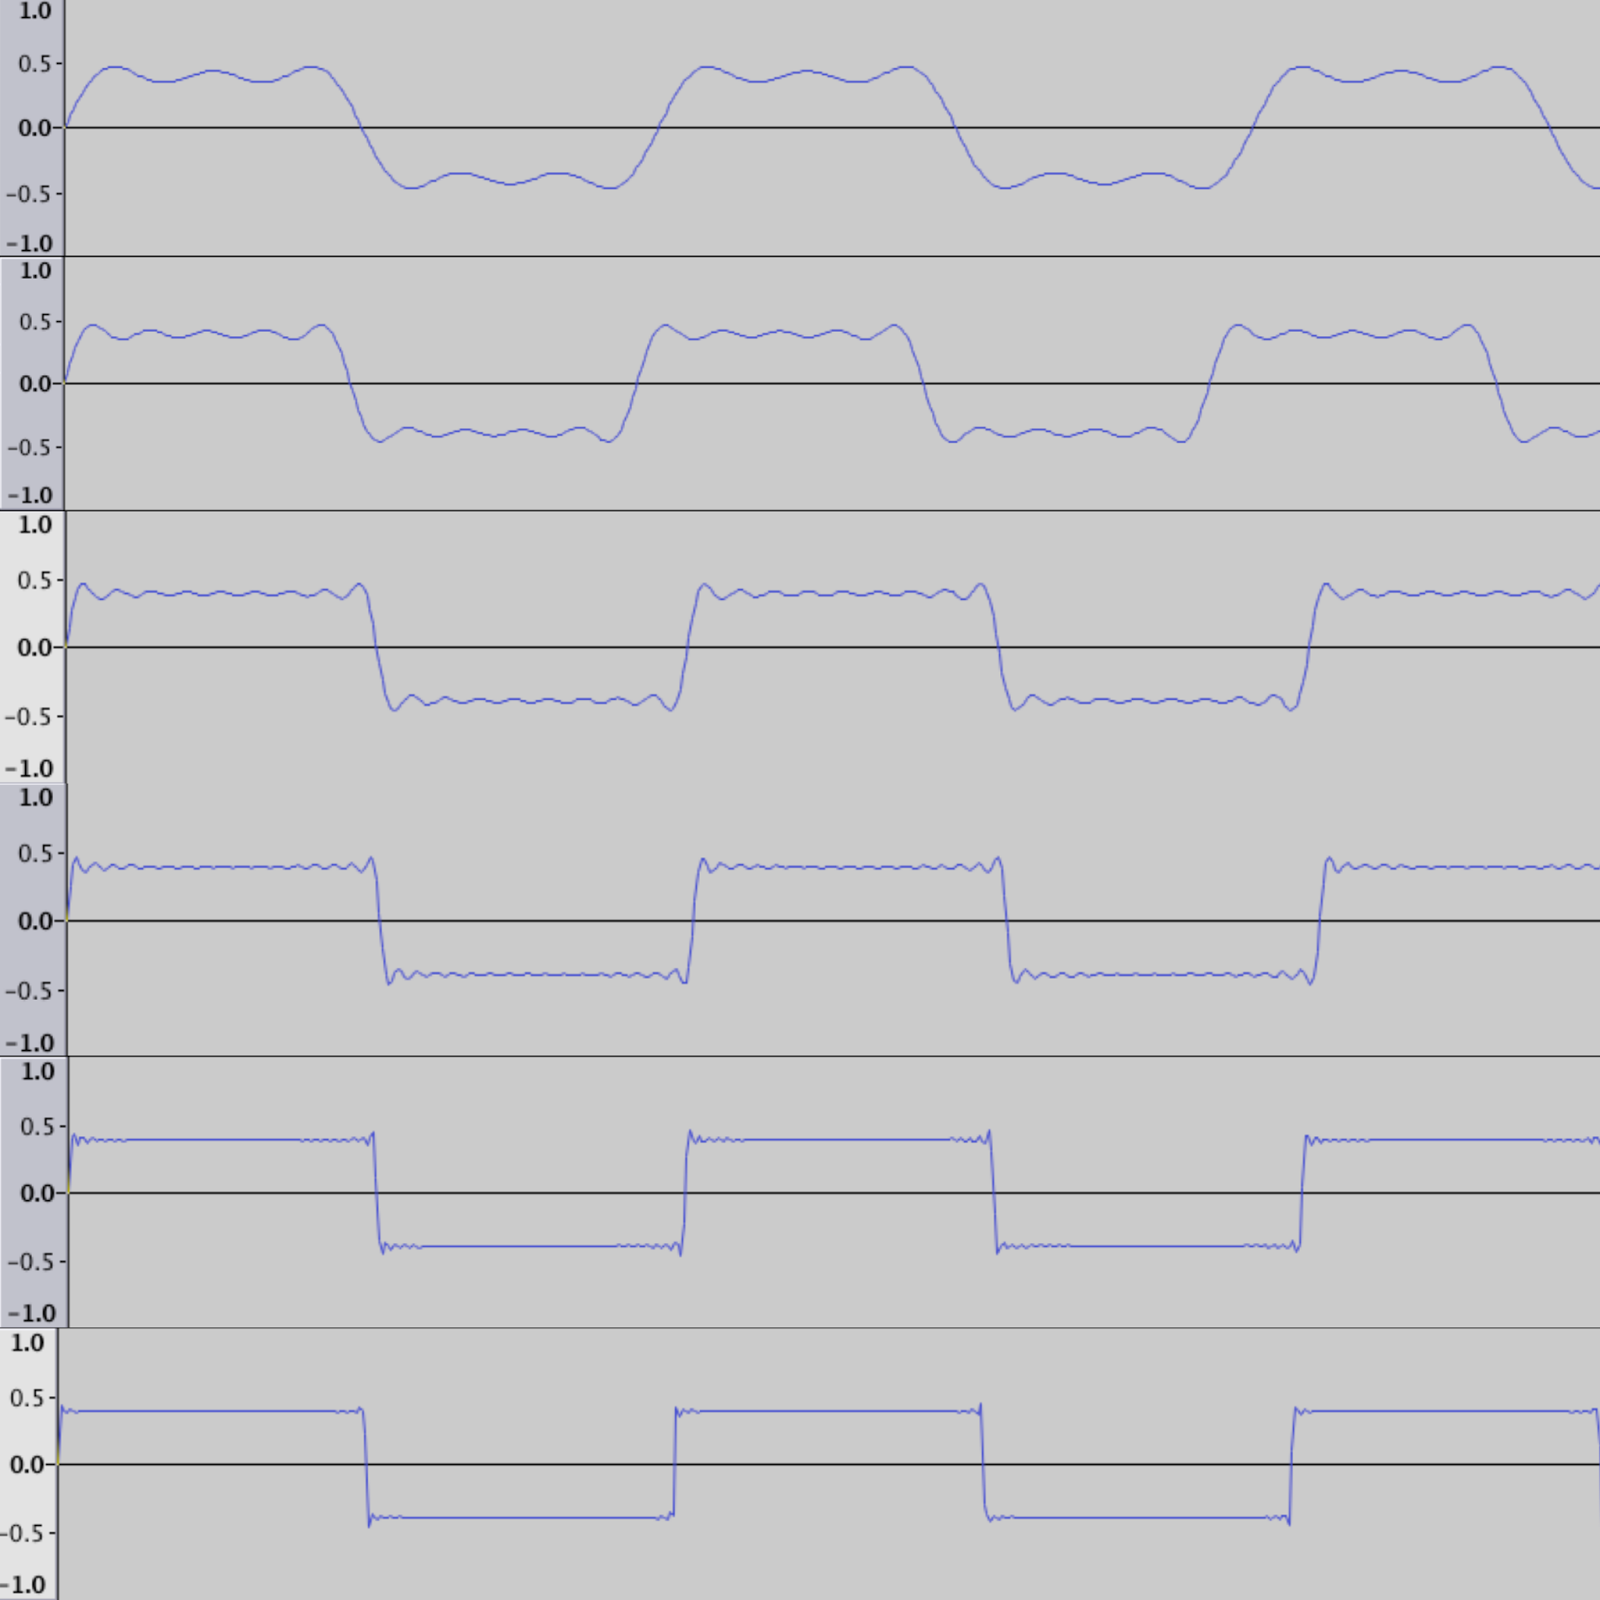
\includegraphics[scale=0.12]{img/square}}

    \ttabbox{\caption{} \label{code:asquare}}{\code{code/asquare.cpp}}

  \end{floatrow}

\end{figure}

\pagebreak

\subsubsection{Sawtooth Waves}

A sawtooth wave is slightly simpler to create through Additive Synthesis, as it requires the summation of every partial rather than only the odd-numbered ones. The respective amplitude is again the reciprocal of the partial number. Equation \ref{eq:asaw} gives a mathematical definition for a sawtooth wave, Figure \ref{fig:saw} displays sawtooth functions with various partial numbers and Table \ref{code:asaw} shows C++ code to generate such functions.

\begin{equation}
  f(t) = \sum\limits_{n=1}^N \frac{1}{n} \sin(\omega n t)
  \label{eq:asaw}
\end{equation}

\begin{figure}[h!]

  \CenterFloatBoxes

  \begin{floatrow}

    \ffigbox{\caption{} \label{fig:saw}}{ 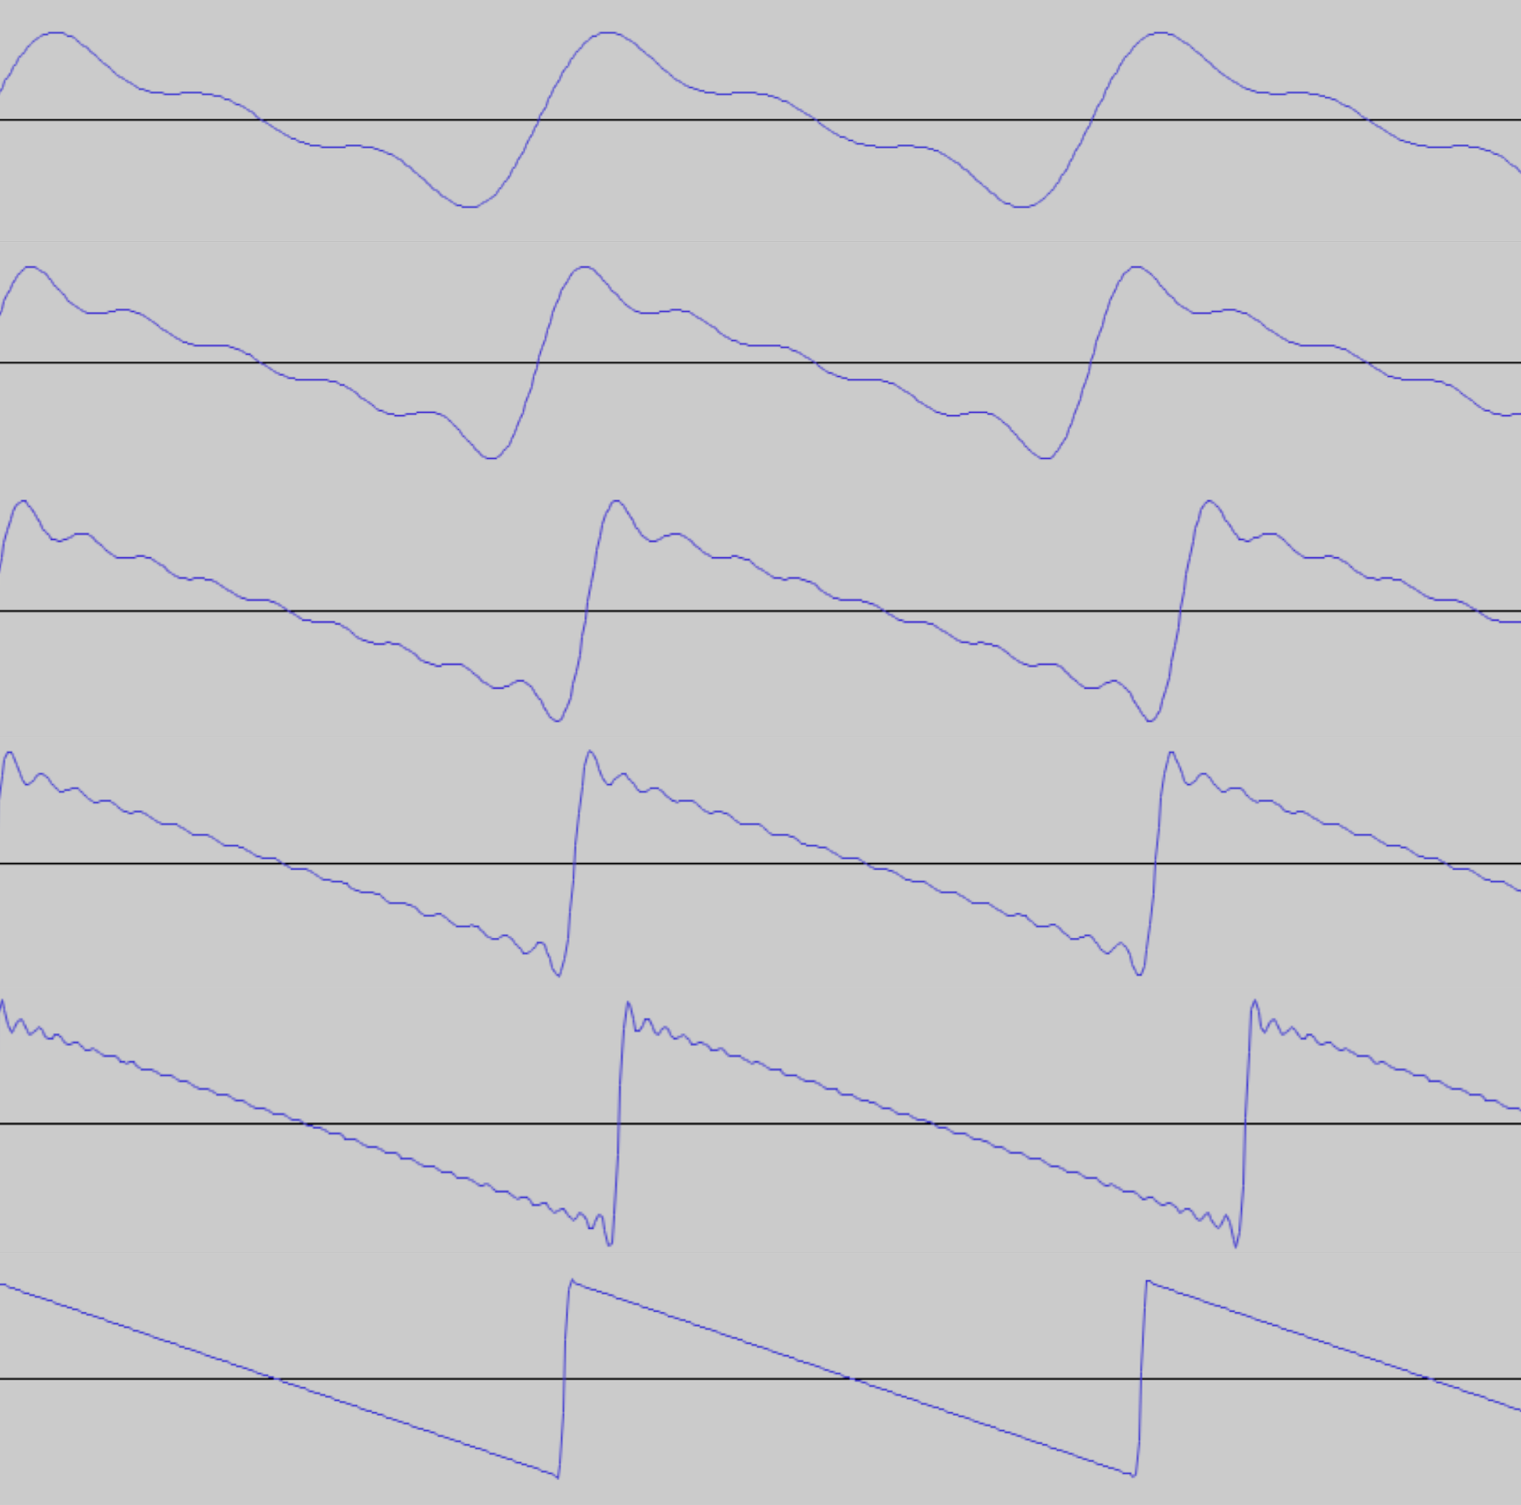
\includegraphics[scale=0.12]{img/saw}}

    \ttabbox{\caption{} \label{code:asaw}}{\code{code/asaw.cpp}}

  \end{floatrow}

\end{figure}

\pagebreak

\subsubsection{Ramp Waves}

Ramp waves are essentially the inverse of sawtooth waves. Therefore, we can simply sum sinusoids as we did for a sawtooth function but change the sign of each partial's amplitude to negative instead of positive. Equation \ref{eq:aramp} gives the mathematical definition, Figure \ref{fig:ramp} displays a set of ramp waveforms with different partial numbers and Table \ref{code:aramp} again shows the accompanying C++ code.

\begin{equation}
  f(t) = \sum\limits_{n=1}^N -\frac{1}{n} \sin(\omega n t)
  \label{eq:aramp}
\end{equation}

\begin{figure}[h!]

  \CenterFloatBoxes

  \begin{floatrow}

    \ffigbox{\caption{} \label{fig:ramp}}{ 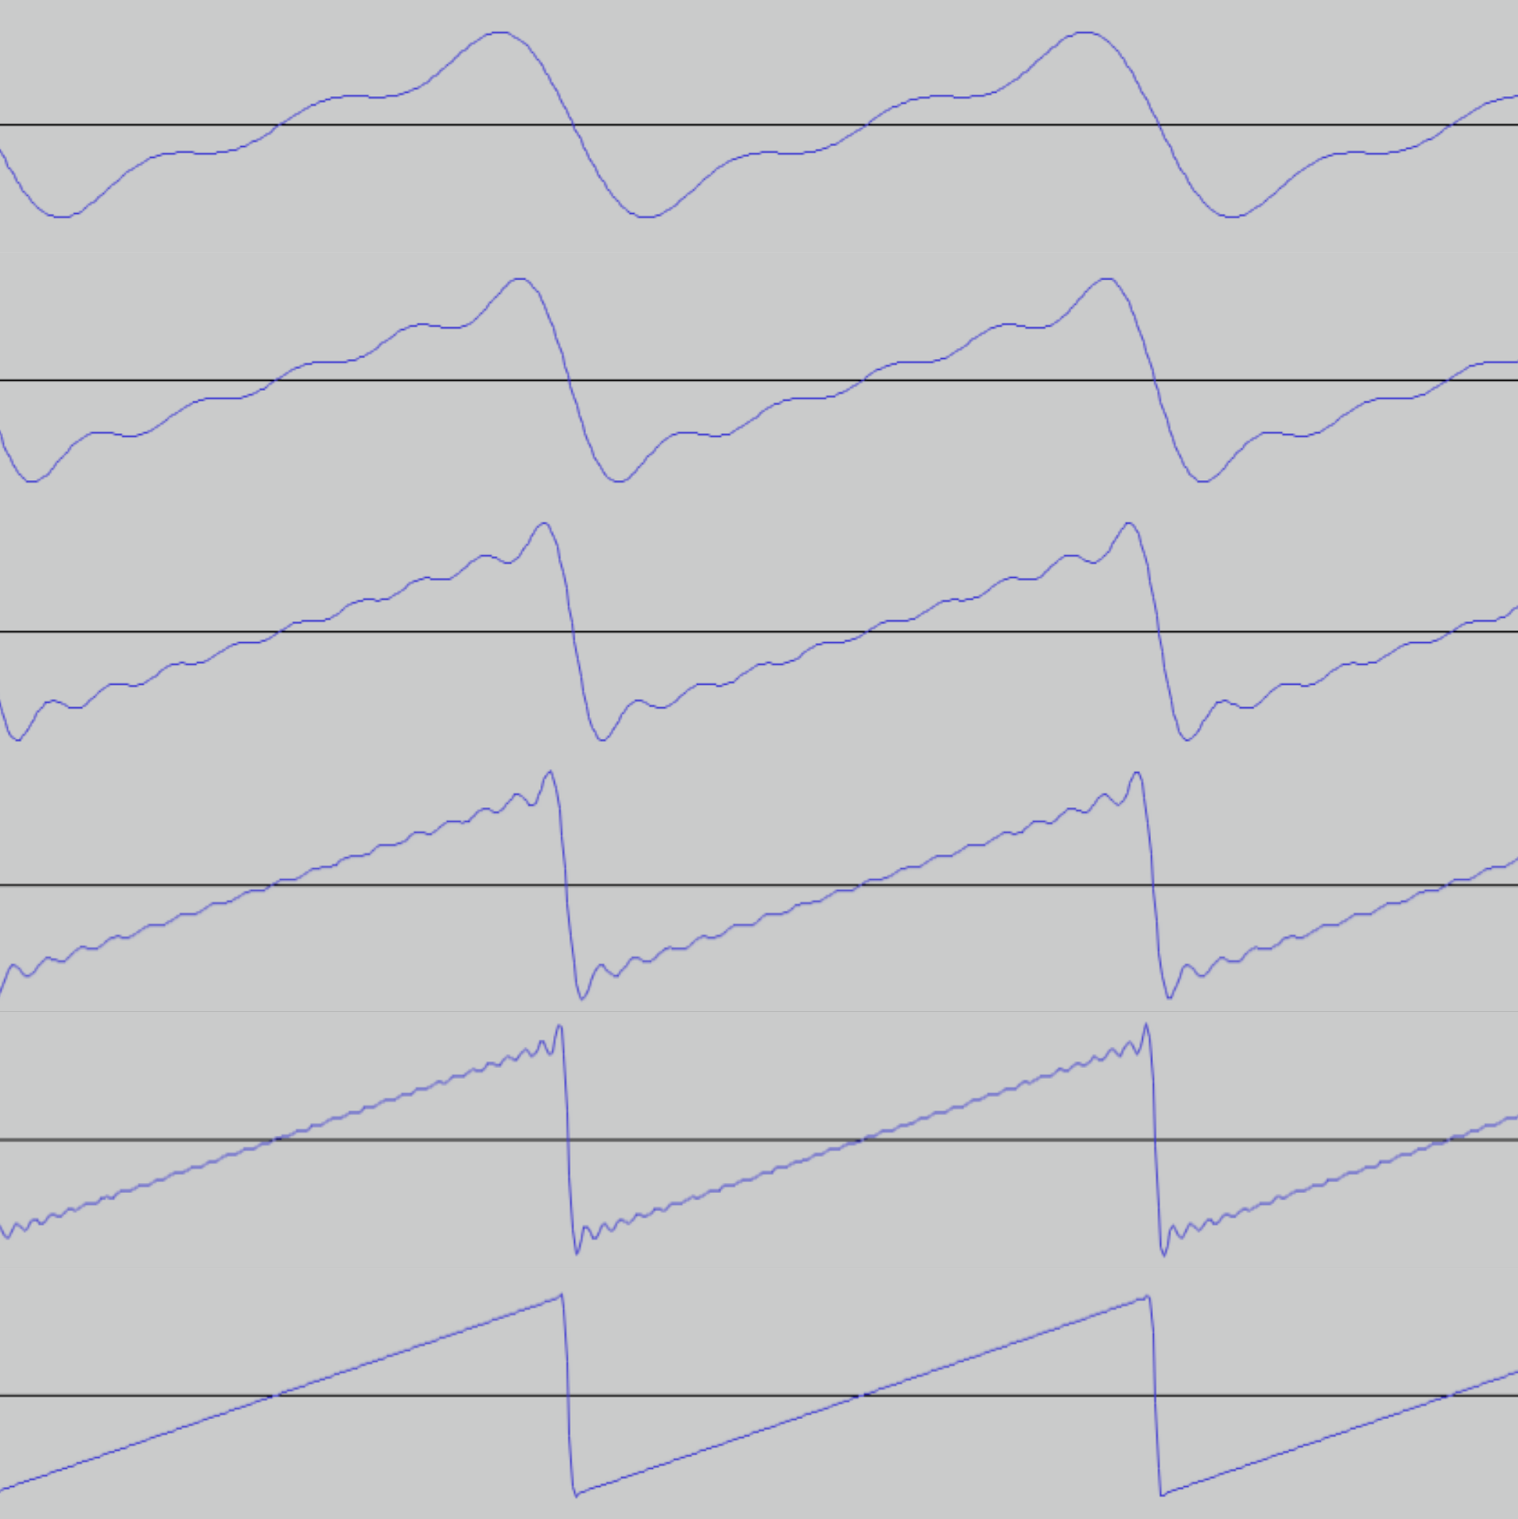
\includegraphics[scale=0.12]{img/ramp}}

    \ttabbox{\caption{} \label{code:aramp}}{\code{code/aramp.cpp}}

  \end{floatrow}

\end{figure}

\subsubsection{Triangle Waves}

The process of generating triangle waves additively differs from previous waveforms. The amplitude of each partial of a triangle waveform is no longer the reciprocal of the partial number, $\frac{1}{n}$, but now the inverse of the partial number squared: $\frac{1}{n^2}$. Moreover, the sign of the amplitude alternates for each partial in the series. As for square waves, only odd-numbered partials are used. Mathematically, such a triangle wave is defined as shown in Equation \ref{eq:atri1} or, more concisely, in Equation \ref{eq:atri2}. Figure \ref{fig:tri} displays such a triangle wave with various partial numbers (2,4,8,16,32 and 64) and Table \ref{code:atri} implements C++ code to compute a triangle wave.

\begin{equation}
  f(t) = \sum\limits_{n=1}^\frac{N}{2} \frac{\sin(\omega (4n-3) t)}{(4n-3)^2} - \frac{\sin(\omega (4n-1) t)}{(4n-1)^2}
  \label{eq:atri1}
\end{equation}

\begin{equation}
  f(t) = \sum\limits_{n=0}^N \frac{(-1)^n}{(2n+1)^2} \sin(\omega (2n + 1) t)
  \label{eq:atri2}
\end{equation}

\begin{figure}

  \CenterFloatBoxes

  \begin{floatrow}

    \ffigbox{\caption{} \label{fig:tri}}{ 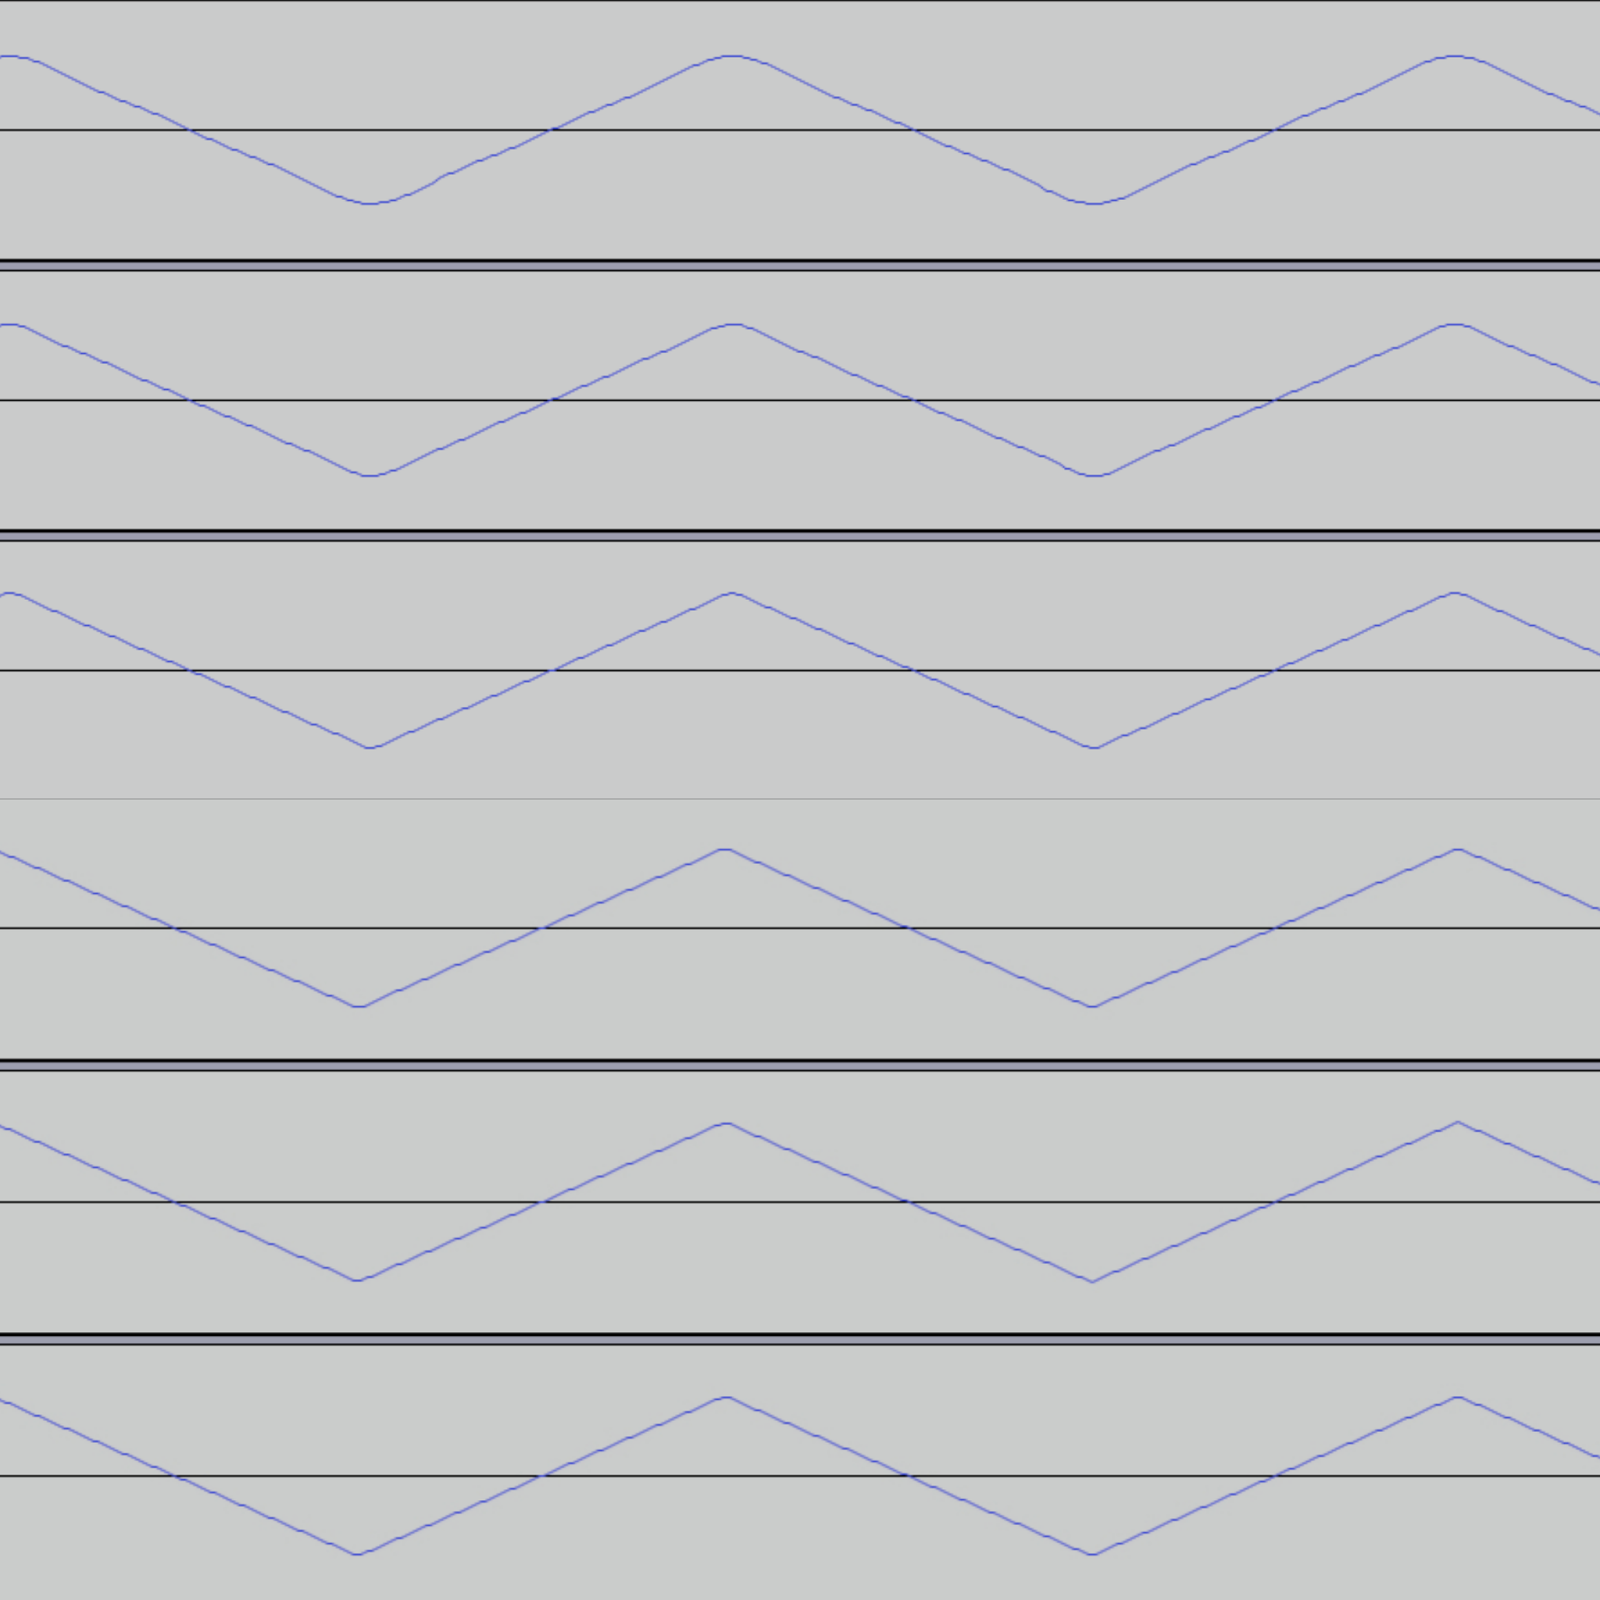
\includegraphics[scale=0.12]{img/tri}}

    \ttabbox{\caption{} \label{code:atri}}{\code{code/atri.cpp}}

  \end{floatrow}

\end{figure}

\section{Real-time calculation versus Wavetable lookup}

Before the generation of more complex waveforms than the sine and cosine waves from section 2.1 can be discussed, the two options for playing back waveforms in a digital synthesis system must be examined: continuous real-time calculation of waveform samples or lookup from a Table that has been calculated once and then written to disk.

\begin{thebibliography}{9}

\bibitem{bsynth}

Daniel R. Mitchell,

\emph{BasicSynth: Creating a Music Synthesizer in Software}.

Publisher: Author.

1st Edition,

2008.

\bibitem{dspguide}

Steven W. Smith,

\emph{The Scientist and Engineer's Guide to Digital Signal Processing}.

California Technical Publishing,

San Diego, California,

2nd Edition,

1999.

\bibitem{sosfm}

Gordon Reid,

\emph{Synth Secrets, Part 12: An Introduction To Frequency Modulation}.

\url{http://www.soundonsound.com/sos/apr00/articles/synthsecrets.htm}

Accessed: 8 October 2014.

\bibitem{samplerates}

Justin Colletti,

\emph{The Science of Sample Rates (When Higher Is Better —-- And When It Isn't)}

2013.\\
  \url{http://www.trustmeimascientist.com/2013/02/04/the-science-of-sample-rates-when-higher-is-better-and-when-it-isnt/}

Accessed: 17 December 2014.

\bibitem{hearing}

John D. Cutnell and Kenneth W. Johnson,

\emph{Physics}.

Wiley,

New York,

4th Edition,

1998.

\end{thebibliography}

\listoffigures

\end{document}
